%
% This is a borrowed LaTeX template file for lecture notes for CS267,
% Applications of Parallel Computing, UCBerkeley EECS Department.
% Now being used for CMU's 10725 Fall 2012 Optimization course
% taught by Geoff Gordon and Ryan Tibshirani.  When preparing 
% LaTeX notes for this class, please use this template.
%
% To familiarize yourself with this template, the body contains
% some examples of its use.  Look them over.  Then you can
% run LaTeX on this file.  After you have LaTeXed this file then
% you can look over the result either by printing it out with
% dvips or using xdvi. "pdflatex template.tex" should also work.
%

\documentclass[twoside]{article}
\setlength{\oddsidemargin}{0.25 in}
\setlength{\evensidemargin}{-0.25 in}
\setlength{\topmargin}{-0.6 in}
\setlength{\textwidth}{6.5 in}
\setlength{\textheight}{8.5 in}
\setlength{\headsep}{0.75 in}
\setlength{\parindent}{0 in}
\setlength{\parskip}{0.1 in}

%
% ADD PACKAGES here:
%

\usepackage{amsmath,amsfonts,graphicx}

%
% The following commands set up the lecnum (lecture number)
% counter and make various numbering schemes work relative
% to the lecture number.
%
\newcounter{lecnum}
\renewcommand{\thepage}{\thelecnum-\arabic{page}}
\renewcommand{\thesection}{\thelecnum.\arabic{section}}
\renewcommand{\theequation}{\thelecnum.\arabic{equation}}
\renewcommand{\thefigure}{\thelecnum.\arabic{figure}}
\renewcommand{\thetable}{\thelecnum.\arabic{table}}

%
% The following macro is used to generate the header.
%
\newcommand{\lecture}[4]{
   \pagestyle{myheadings}
   \thispagestyle{plain}
   \newpage
   \setcounter{lecnum}{#1}
   \setcounter{page}{1}
   \noindent
   \begin{center}
   \framebox{
      \vbox{\vspace{2mm}
    \hbox to 6.28in { {\bf EE302 - Feedback Systems
	\hfill Spring 2019} }
       \vspace{4mm}
       \hbox to 6.28in { {\Large \hfill Lecture #1 \hfill} }
       \vspace{2mm}
       \hbox to 6.28in { {\it Lecturer: #2 \hfill } }
      \vspace{2mm}}
   }
   \end{center}
   \markboth{Lecture #1}{Lecture #1}

   \vspace*{4mm}
}
%
% Convention for citations is authors' initials followed by the year.
% For example, to cite a paper by Leighton and Maggs you would type
% \cite{LM89}, and to cite a paper by Strassen you would type \cite{S69}.
% (To avoid bibliography problems, for now we redefine the \cite command.)
% Also commands that create a suitable format for the reference list.
\renewcommand{\cite}[1]{[#1]}
\def\beginrefs{\begin{list}%
        {[\arabic{equation}]}{\usecounter{equation}
         \setlength{\leftmargin}{2.0truecm}\setlength{\labelsep}{0.4truecm}%
         \setlength{\labelwidth}{1.6truecm}}}
\def\endrefs{\end{list}}
\def\bibentry#1{\item[\hbox{[#1]}]}

%Use this command for a figure; it puts a figure in wherever you want it.
%usage: \fig{NUMBER}{SPACE-IN-INCHES}{CAPTION}
\newcommand{\fig}[3]{
			\vspace{#2}
			\begin{center}
			Figure \thelecnum.#1:~#3
			\end{center}
	}
% Use these for theorems, lemmas, proofs, etc.
\newtheorem{theorem}{Theorem}[lecnum]
\newtheorem{lemma}[theorem]{Lemma}
\newtheorem{proposition}[theorem]{Proposition}
\newtheorem{claim}[theorem]{Claim}
\newtheorem{corollary}[theorem]{Corollary}
\newtheorem{definition}[theorem]{Definition}
\newenvironment{proof}{{\bf Proof:}}{\hfill\rule{2mm}{2mm}}

% **** IF YOU WANT TO DEFINE ADDITIONAL MACROS FOR YOURSELF, PUT THEM HERE:

\begin{document}

% Lecture Details
\lecture{5}{Asst. Prof. M. Mert Ankarali}

\par 

\section{DC Motor Modeling}

A generel ``ideal'' DC motor can be moddled as in the Figure below.

  \begin{minipage}[h]{1\linewidth}
    \begin{center}
      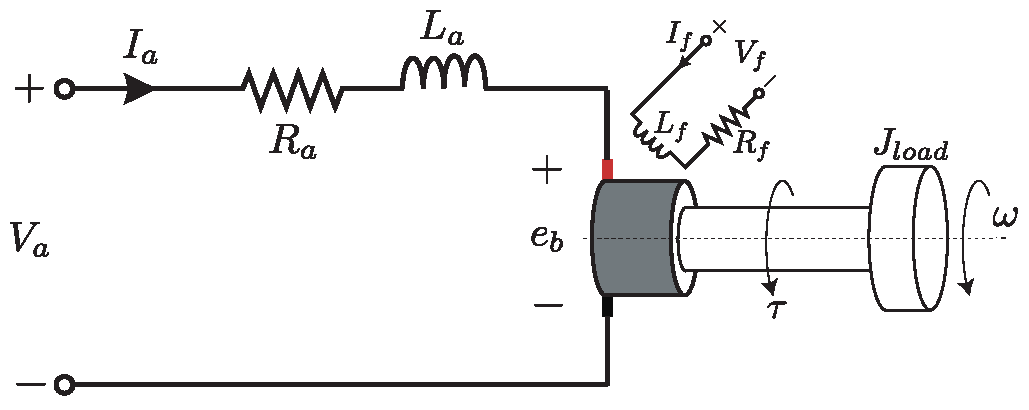
\includegraphics[width=0.9\textwidth]{DC_Motor}
    \end{center}
  \end{minipage}
 
The dependent and ``independent'' variables associated with the idealized DC motor model and
important relations/equations regarding the electro-mechanical interactions are given below.

\vspace{12pt}

  \begin{minipage}[h]{0.5\linewidth}
    \begin{center}
\begin{tabular}{| l | l |}
\hline
$V_a$ & Armature voltage  \\
$i_a$ & Armature current  \\
$V_f$ &  ``Field voltage'' \\
$i_f$ &  ``Field current'' \\
$V_b$ & Back emf \\
$\omega$ & Rotor angular velocity \\
$\tau$ & Generated torque \\
$\Phi$ & Air-gap magnetic flux \\
\hline
\end{tabular}
    \end{center}
  \end{minipage}
  \begin{minipage}[h]{0.5\linewidth}
\begin{align*}
	\Phi(t) &= K_f I_f(t) 
	\\
	\tau(t) &= K_m \Phi(t) I_a(t)
	\\
	e_b(t) &= K_b \omega(t)
\end{align*}
  \end{minipage}  
  
\vspace{12pt}
%
Note that if both $i_f(t)$ and $i_a(t)$ are non-constant the electric-motor model 
won't be LTI. In order to have an LTI representation, there are two options
%
\begin{itemize}
	\item Armature controlled DC motor: $\Phi$ is kept constant 
	%
	\begin{align*}
		\tau(t) &= K_m \Phi I_a(t) = K_{\tau}^a I_a(t)
	\end{align*}
	%
	\item Field controlled DC motor: $i_a$ is kept constant 
	%
	\begin{align*}
		\tau(t) &= K_m K_f I_a I_f(t) = K_{\tau}^f I_f(t)
	\end{align*}
	%
\end{itemize}

\subsection{Armature Controlled DC Motor}

Majority of ``DC'' Motors are controlled (and indeed manufactured) with this approach. Either
there is a permanent magnet which satisfies the constant $\Phi$ or a constant current is supplied
through the coils that generates the magnetic field.

Let's model the following electro-mechanical system where the DC motor is armature controlled 
and given that $y(t) = \omega(t)$ and $u(t) = V_a(t)$.

  \begin{minipage}[h]{1\linewidth}
    \begin{center}
      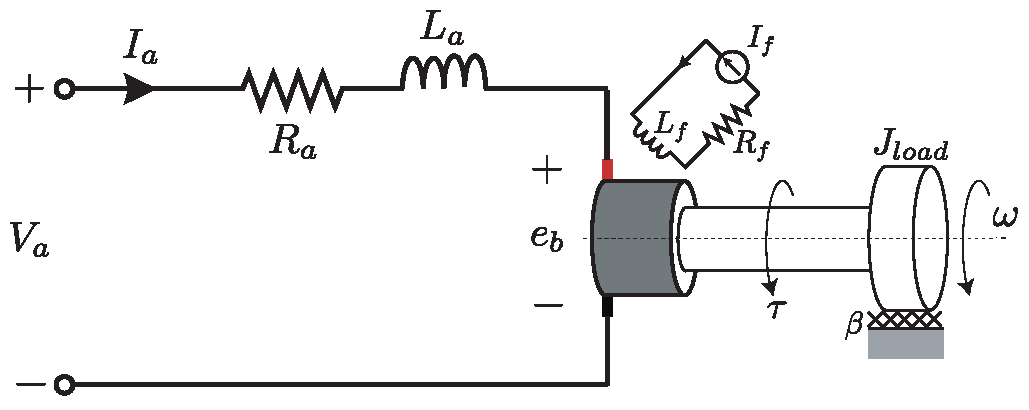
\includegraphics[width=0.9\textwidth]{Armature_DC_Motor}
    \end{center}
  \end{minipage} 
 
 We already know the transfer function of the mechanical sub system:
 %
\begin{align*}
	\Omega(s) &= \frac{1}{J s + \beta} \mathcal{T}(s)
\end{align*}
 %
 Now let's write the remaining equations in Laplace domain
 %
 \begin{align*}
	I_a(s) &= \frac{1}{L_a s + R_a} \left( V_a(s) - E_b(s) \right)
	\\
	\mathcal{T}(s) &= K_a I_a(s)
	\\
	E_b(s) &= K_b \Omega(s)
\end{align*}
%
where $K_a \equiv K_{\tau}^a$. Now let's build a block-diagram topology

  \begin{minipage}[h]{1\linewidth}
    \begin{center}
      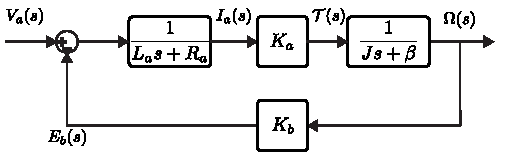
\includegraphics[width=0.75\textwidth]{arm_block}
    \end{center}
  \end{minipage} 
  
  If we simplify the block diagram, we obtain the transfer function form
   %
   \begin{align*}
   	G(s) &= \frac{\Omega(s)}{V_a(s)} = \frac{\frac{K_a}{(L_a s + R_a) (J s + \beta)} }{1 + \frac{K_a K_b}{(L_a s + R_a) (J s + \beta)}}
	\\
	&= \frac{K_a}{L_a J s^2 + ( L_a \beta + R_a J ) s + R_a \beta
          + K_a K_b}
   \end{align*}
   %
   \textbf{Example 1:} Given that $V_a$ is the input and $\theta$ is the output, construct a block-diagram for the following electro mechanical system and then compute the transfer function.
  
    \begin{minipage}[h]{1\linewidth}
    \begin{center}
      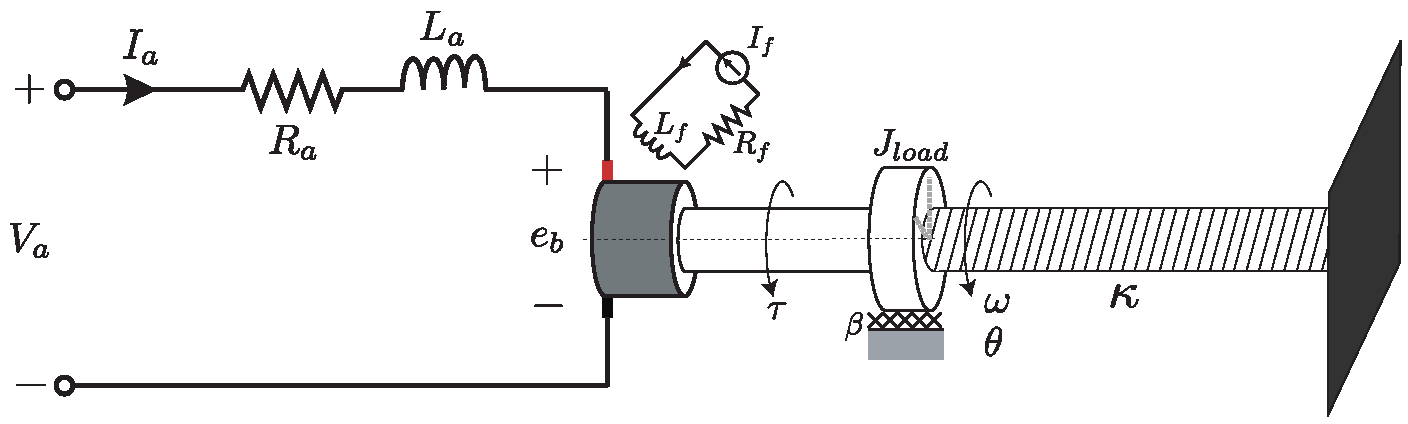
\includegraphics[width=1\textwidth]{DC_Mot_ex1}
    \end{center}
  \end{minipage} 
  
    \textbf{Solution:} A block diagram topology can be constructed by modifying the previous block diagram (armature controlled DC motor without torsional spring).
  
    \begin{minipage}[h]{1\linewidth}
    \begin{center}
      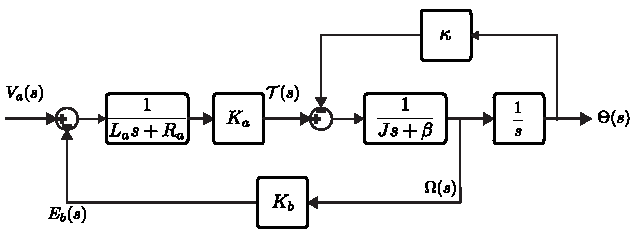
\includegraphics[width=1\textwidth]{block_ex1}
    \end{center}
  \end{minipage} 
  
  Then the transfer function can ne derived using block-diagram simplification methods as given in the next page
  
      \begin{minipage}[h]{1\linewidth}
    \begin{center}
      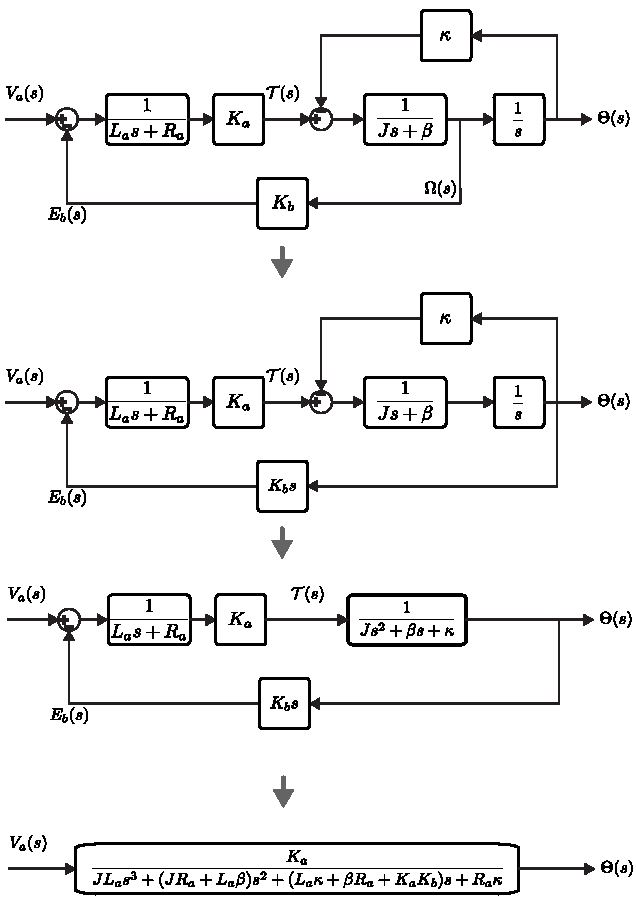
\includegraphics[width=1\textwidth]{block_ex1_simplify}
    \end{center}
  \end{minipage} 
  
  \subsection{Field Controlled DC Motor}
%
In the field controlled DC motors, magnetic flux is actively controlled by adjusting
electrical current/voltage. We assume that $I_a$ is constant (LTI constraints). Since,
there is no ``feedback'' in this field controlled DC motor model, the electrical circuit
is isolated from the mechanical one. 

Let's model the following electro-mechanical system where the DC motor is field controlled 
and given that $y(t) = \omega(t)$ and $u(t) = V_f(t)$.

  \begin{minipage}[h]{0.65\linewidth}
    \begin{center}
      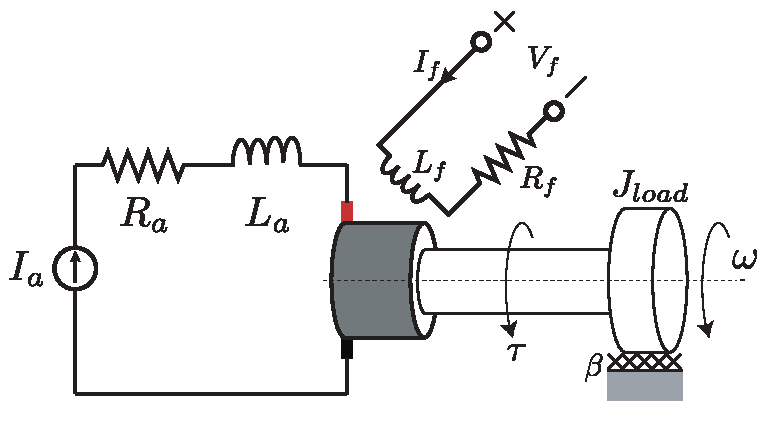
\includegraphics[width=0.95\textwidth]{Field_DC_Motor}
    \end{center}
  \end{minipage}
  %
   \begin{minipage}[h]{0.45\linewidth}
    \begin{center}
      \begin{align*}
            \frac{\Omega(s)}{\mathcal{T}(s)} &= \frac{1}{J s + \beta}
            \\
            \frac{I_f(s)}{V_f(s)} &= \frac{1}{L_f s + R_f}
            \\
            \mathcal{T}(s) &= K_f I_f(s)
\end{align*}
    \end{center}
  \end{minipage}

where $K_f \equiv K_{tau}^f$. Finally transfer function can be computed as
\begin{align*}
            G(s) &= \frac{K_f}{ J L_f s^2 +  (J R_f + \beta L_f) s + ( \beta R_f + K_f)}
\end{align*}
    %
     \textbf{Example 2:} Consider the following closed-loop field controlled electro-mechanical circuit. It is given that $\theta^*(t)$, i.e.
     reference angle signal, is the input and $\theta_2$, angular displacement of the second gear, is the output. In the
     system, there is an encoder which reads the angular displacement and sends it to a controller box. The other input of this box is 	the reference signal. The box produces an output voltage, $V_c = \gamma \left( \theta^* - \theta_2 \right)$, and feeds it to the 
     input terminal of the $V_f$. Compute the transfer function.
  
  
    \begin{minipage}[h]{1\linewidth}
    \begin{center}
      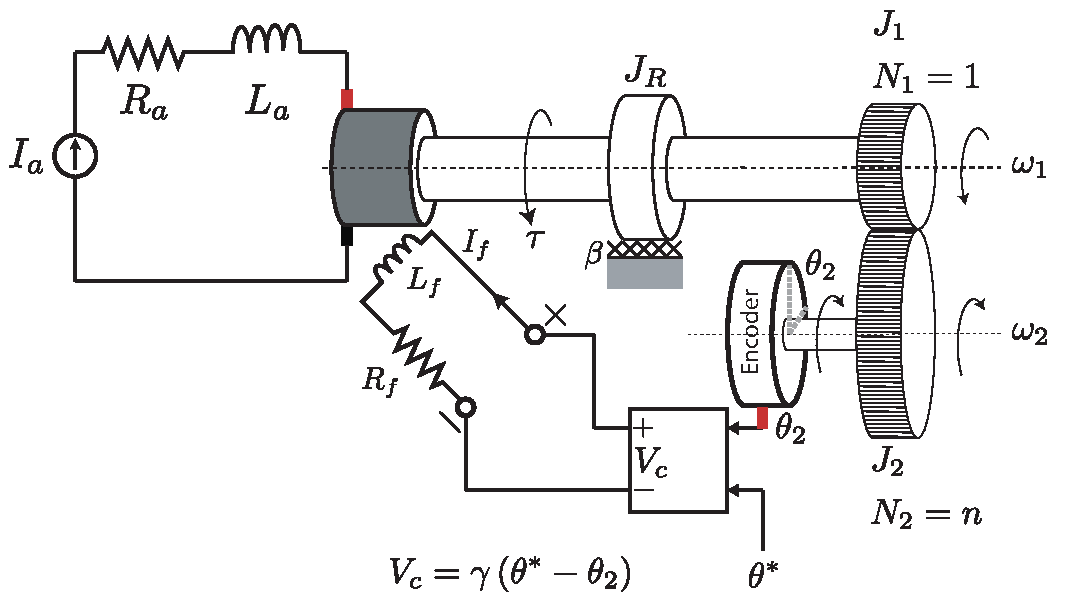
\includegraphics[width=0.9\textwidth]{DC_Mot_ex2}
    \end{center}
  \end{minipage} 
  
    \textbf{Solution:} A block diagram topology can be constructed by modifying the previous block diagram (armature controlled DC motor without torsional spring).
    
    Let's first find a transfer function from $\tau$ to $\omega_2$ and $\theta_2$. The easiest way of computing this is using the concept of reflected inertia, damping, and torque. 
    %
    \begin{align*}
            \Omega_2(s) &= \frac{\bar{\mathcal{T}}(s)}{J_T s + \beta_T } = \frac{n}{\left( n^2 J_R + n^2 J_1 + J2 \right) s + n^2 \beta } 	\mathcal{T}(s) 
            \\
            \Theta_2(s) &= \frac{n \mathcal{T}(s)}{J_T s^2 + \beta_T s} 
    \end{align*}
    %
    We know that Laplace domain equations for remaining parts take the form
    %
    \begin{align*}
    \frac{\mathcal{T}(s)}{V_f(s)} &= \frac{K_f}{L_f s + R_f}
    \\
    V_f(s) &= \gamma \left( \Theta^*(s) - \Theta_2(s) \right)
    \end{align*}
    %
    Now let's construct a block diagram representation
    
        \begin{minipage}[h]{1\linewidth}
    \begin{center}
      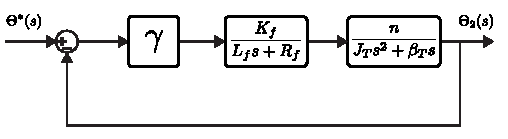
\includegraphics[width=0.75\textwidth]{field_block}
    \end{center}
  \end{minipage} 
    
Finally, transfer function can be computed as
    %
    \begin{align*}
            G(s) &= \frac{\gamma K_f n}{ J_T L_f s^3 +  (J_T R_f + \beta_T L_f) s^2 + \beta_T R_f s + \gamma K_f n}
\end{align*}
    
% **** This ENDS THE EXAMPLES. DON'T DELETE THE FOLLOWING LINE:
\end{document}